\documentclass[11pt]{beamer}
\usetheme{Rochester}
\usepackage[utf8]{inputenc}
\usepackage{amsmath}
\usepackage{amsfonts}
\usepackage{amssymb}
\usepackage{graphicx}
%\author{}
%\title{}
%\setbeamercovered{transparent} 
%\setbeamertemplate{navigation symbols}{} 
%\logo{} 
%\institute{} 
%\date{} 
%\subject{} 
\begin{document}

\begin{frame}
\title{Computational Astrophysics}
\author{E. Larrañaga}
\institute{Observatorio Astronómico Nacional\\
Universidad Nacional de Colombia}
\titlepage
\end{frame}

\begin{frame}{Outline}
\tableofcontents
\end{frame}

\section{Sources of Error}

\subsection{Round-off Error}
\begin{frame}[fragile]{Round-off Error}
Round-off error arises from the error inherent in representing a floating point number with a finite number of bits in the computer.
\end{frame}


\begin{frame}[fragile]{Round-off Error}
\tiny
\begin{semiverbatim}
""" 
Round-off Error
We find the value of epsilon for which 1. + epsilon = 1.

This gives the machine epsilon value, representing the error inherent to
representing a floating point number
"""

epsilon = 1. # Initial value for epsilon

while (1. + epsilon != 1.):
    epsilon = epsilon /2.

print (epsilon)
 
#Iterates, halving epsilon until 1 + epsilon = 1
# Prints the value of the machine epsilon
\end{semiverbatim}
\normalsize
\end{frame}

\subsection{Truncation Error}
\begin{frame}[fragile]{Truncation Error}
\normalsize
Truncation error is a feature of an algorithm. \\
\bigskip

Typically we expand the expressions about some small quantity. When throwing away higher-order terms, there is a truncation in the expression.\\
\bigskip

This introduces an error in the representation !!.\\
\bigskip

 If the quantity we expand about truly is small, then the error is small.
\end{frame}

\begin{frame}[fragile]{Convergence Test}
\textbf{Example:}\\
Function:
\begin{equation}
f(x) = \sin (x)
\end{equation}

Taylor series representation:
\begin{equation}
f(x) = \sum_{n=1}^\infty (-1)^{n-1} \frac{x^{2n-1}}{(2n-1)!}
\end{equation}

Truncation for $ \left| x \right| \ll 1 $:
\begin{equation}
f(x) = x - \frac{x^3}{6} + \mathcal{O} (x^5)
\end{equation}
\end{frame}

\begin{frame}[fragile]{Convergence Test}
\tiny
\begin{semiverbatim}
""" 
Truncation Error - Convergence Test
We implement a 5th order accurate approximation of the function Sin(x)

We define a procedure that calculates the difference between the value of 
the Sin(x) function and the truncated approximation. 

Calculating the value of this epsilon for x<1 and then taking half of 
this value of x we show that the epsilon reduces by 2**5 = 32, 
demonstrating 5th-order accuracy
"""

import math as m
 
# Definition of the function giving the truncation error
def epsilon(x):
    return m.sin(x) - (x - (x**3)/6)

# Value to calculate the function
x = 0.1

# Results. We use the formating in the print function to show the results
print("\\nFor x = \%f the value of the truncation error is epsilon = \%e" \%( x, epsilon(x)))
print("For x = \%f the value of the truncation error is epsilon = \%e" \%( x/2, epsilon(x/2)))
print("")
print("The ratio of these values is \%f " \%(epsilon(x)/epsilon(x/2)))
\end{semiverbatim}
\end{frame}

\section{Finite Differences}
\subsection{Differentiation of a Discrete Function}
\begin{frame}[fragile]{Differentiation of a Discrete Function}
Collection of equally spaced points $x_i$ (such that $\Delta x = x_{i+1} - x_i$) and the corresponding values $f_i$. The derivative of this discrete function can be calculated using
\pause
\begin{equation}
\left. \frac{df}{dx} \right|_i = \frac{f_i - f_{i-1}}{\Delta x} 
\end{equation}
or using
\begin{equation}
\left. \frac{df}{dx} \right|_i = \frac{f_{i+1} - f_i}{\Delta x}. 
\end{equation}

These finite difference derivatives are first order accurate.\\
\pause
A second order accurate method to calculate this derivative uses the centered difference
\pause
\begin{equation}
\left. \frac{df}{dx} \right|_i = \frac{f_{i+1} - f_{i-1}}{2 \Delta x}. 
\end{equation}
\end{frame}

\subsection{Differentiation of an Analytic Function}
\begin{frame}[fragile]{Differentiation of an Analytic Function}
Numerically find the derivative of an analytic function $f(x)$
\pause
\begin{equation}
f'(x_0) = \left. \frac{df}{dx} \right|_{x_0} = \lim_{\Delta x \rightarrow 0} \frac{\Delta f}{\Delta x} (x_0)
\end{equation}
\pause
Taylor expansion
\begin{eqnarray}
f(x_0 + \delta x) &=& \sum_{n=0}^\infty \frac{f^{(n)} (x_0)}{n!} \delta x^n \\
                 &=& f(x_0) +  f'(x_0) \delta x + \mathcal{O} (\delta x^2)
\end{eqnarray}
\end{frame}

\begin{frame}[fragile]{Differentiation}
\begin{equation}
\left. \frac{df}{dx} \right|_{x_0} = \frac{f(x_0 + \delta x) - f(x_0)}{\delta x} + \mathcal{O} (\delta x)
\end{equation}
\pause
\begin{center}
\textit{Forward difference} estimate for $f'(x_0)$
\end{center} 
\end{frame}

\begin{frame}[fragile]{Differentiation of an Analytic Function}
\begin{figure}
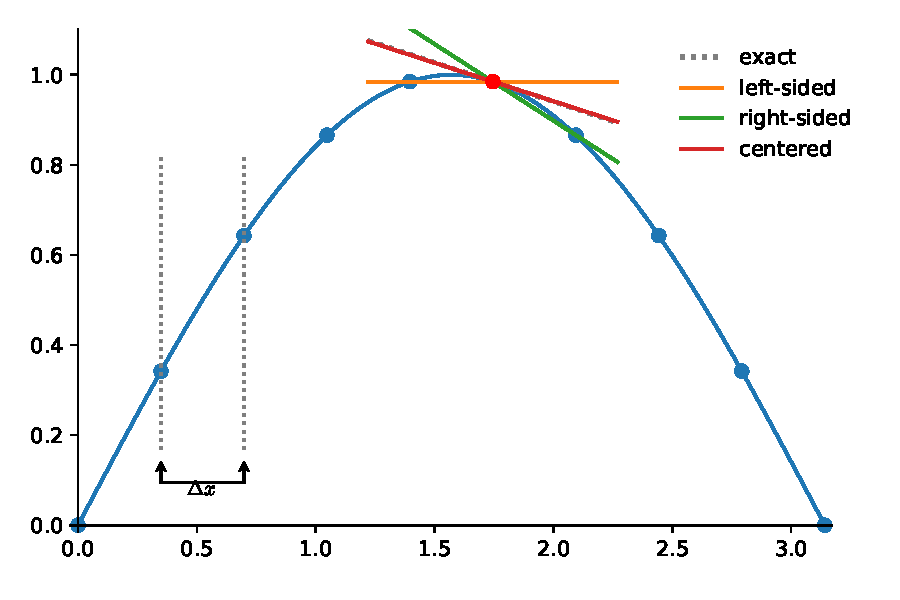
\includegraphics[scale=0.6]{derivatives.pdf}
\end{figure}
\end{frame}

\begin{frame}[fragile]{Differentiation of an Analytic Function}
\begin{equation}
f'(x_0) = \frac{f(x_0 + \delta x) - f(x_0)}{\delta x} + \mathcal{O} (\delta x)
\end{equation}
\begin{center}
First order \textit{forward difference} estimate for $f'(x_0)$
\end{center} 

\begin{equation}
f'(x_0) = \frac{f(x_0) - f(x_0 - \delta x)}{\delta x} + \mathcal{O} (\delta x)
\end{equation}
\begin{center}
First order \textit{backward difference} estimate for $f'(x_0)$
\end{center} 

\begin{equation}
f'(x_0) = \frac{f(x_0 + \delta x) - f(x_0 - \delta x)}{2\delta x} + \mathcal{O} (\delta x^2) \label{eq:secondOrder}
\end{equation}
\begin{center}
Second order \textit{central difference} estimate for $f'(x_0)$
\end{center} 
\end{frame}

\begin{frame}[fragile]{Differentiation of an Analytic Function}
An optimal value for $\delta x$ requires a balance of truncation error (which needs a small $\delta x$) and the round-off error (which becomes large when $\delta x$ is close to the machine $\epsilon$ ).\\
\bigskip

\pause
A rule-of-thumb for the election is $\delta \approx \sqrt{\epsilon}$.
\end{frame}

\begin{frame}[fragile]{Differentiation of an Analytic Function in an Unevenly Spaced Grid}
Equidistant grids are the conceptually simplest way of discretizing a
problem. \\
\bigskip
\pause
They are, however, in many cases by far not the most
efficient way, since many problems need more resolution in some parts
of their domain than in others. \\
\bigskip
\pause
 
For example, when modeling the stellar
collapse of an iron core to a neutron star it is useful to resolve the steep density
gradients near the neutron star. In this process, a resolution of order $100\,\mathrm{m}$
is required within $\sim 30\,\mathrm{km}$ of the origin, while a cell size
of order 10 km is sufficient at radii above $\sim$1000\,km. \\
\end{frame}


\begin{frame}[fragile]{Differentiation of an Analytic Function in an Unevenly Spaced Grid}
\small

We want to evaluate $f'(x)$ at $x = x_i$. \\
Consider the steps $\delta x_1 = x_i - x_{i-1}$
and $\delta x_2 = x_{i+1} - x_i$.\\

\pause
Then,
\begin{equation}
\begin{aligned}
f(x_i + \delta x_2) &= f(x_i) + \delta x_2 f'(x_i) + \frac{\delta x_2^2}{2} f''(x_i) +
\mathcal{O}(\delta x_2^3) \\
f(x_i - \delta x_1) &= f(x_i) - \delta x_1 f'(x_i) + \frac{\delta x_1^2}{2} f''(x_i) +
\mathcal{O}(\delta x_1^3) 
\end{aligned}
\end{equation}

\pause

Eliminating $f''(x_i)$ and solving for $f'(x_i)$,
\begin{equation}
\begin{aligned}
f'(x_i) &= \frac{\delta x_1}{\delta x_2(\delta x_1+\delta x_2)} f(x_{i+1}) - \frac{\delta x_1 - \delta x_2}{\delta x_2 \delta x_1} f(x_i)
- \frac{\delta x_2}{\delta x_1(\delta x_1 + \delta x_2)} f(x_{i-1}) \,.
\end{aligned}
\end{equation}
\pause
If $\delta x_1 = \delta x_2 = \delta x$ this reduces to the standard difference equation (\ref{eq:secondOrder}).
\normalsize
\end{frame}


\end{document}